\documentclass[11pt]{article}
\usepackage{amsmath,amsfonts,latexsym,graphicx}
\usepackage{fullpage,color}
%\usepackage{text}
%\usepackage{algo}
\usepackage{url,hyperref}
\usepackage{complexity}
\usepackage[linesnumbered,boxed,ruled,vlined]{algorithm2e}

\pagestyle{empty}

\setlength{\oddsidemargin}{0in}
\setlength{\topmargin}{0in}
\setlength{\textwidth}{6.5in}
\setlength{\textheight}{8.5in}

\newtheorem{fact}{Fact}
\newtheorem{lemma}{Lemma}
\newtheorem{theorem}[lemma]{Theorem}
\newtheorem{defn}[lemma]{Definition}
\newtheorem{assumption}[lemma]{Assumption}
\newtheorem{corollary}[lemma]{Corollary}
\newtheorem{prop}[lemma]{Proposition}
\newtheorem{exercise}[lemma]{Exercise}
\newtheorem{claim}[lemma]{Claim}
\newtheorem{remark}[lemma]{Remark}
\newtheorem{prob}{Problem}
\newtheorem{conjecture}{Conjecture}

\newenvironment{note}[1]{\medskip\noindent \textbf{#1:}}%
        {\medskip}

\newenvironment{proof}{\vspace{-0.05in}\noindent{\bf Proof:}}%
        {\hspace*{\fill}$\Box$\par}
\newenvironment{proofsketch}{\noindent{\bf Proof Sketch.}}%
        {\hspace*{\fill}$\Box$\par\vspace{4mm}}
\newenvironment{proofof}[1]{\smallskip\noindent{\bf Proof of #1.}}%
        {\hspace*{\fill}$\Box$\par}

\newcommand{\etal}{{\em et al.}\ }
\newcommand{\assign}{\leftarrow}

\newcommand{\opt}{\textrm{\sc OPT}}
\newcommand{\script}[1]{\mathcal{#1}}
\newcommand{\ceil}[1]{\lceil #1 \rceil}
\newcommand{\floor}[1]{\lfloor #1 \rfloor}
\newtheorem{problem}{Problem}
\renewcommand{\R}{\mathcal{R}}

\begin{document}

\setlength{\fboxrule}{.5mm}\setlength{\fboxsep}{1.2mm}
\newlength{\boxlength}\setlength{\boxlength}{\textwidth}
\addtolength{\boxlength}{-4mm}
\begin{center}\framebox{\parbox{\boxlength}{\bf
IIIS 2014 Spring: ATCS - Selected Topics in Optimization \\
Lecture date: ADD DATE, 2009\\
Instructor: Jian Li   \hfill Scribe: YOUR NAME}}\end{center}
\vspace{5mm}

\section{Recap}
Recall the following definition about $\epsilon$-net:
A range space $(X;R)$ is a pair consisting of an underlying universe X of objects, and a certain collection
	R of subsets (ranges) of X. 
Furthermore, we focus on those range spaces of finite  VC-dimension; namely, for any finite subset $P\subset X$, the number of distinct sets $r\cap P$,
for $r\in R$, is $O(|P|^d)$, for some constant $d$ (which is upper bounded by the VC-dimension of $(X;R)$).

Then given a range space $(X;R)$, a finite subset $P \subset X$, and a parameter $0 < \epsilon < 1$, an $\epsilon$-net for $P$ (and
$R$) is a subset $N \subseteq P$ with the property that any range $r \in R$ with $|r\cap P|\geq \epsilon|P|$ contains an element
of $N$. 

By last lecture, we have known that for any $(X;R)$, finite subset $P\subset X$ and $\epsilon$, such
	that $(X;R)$ has finite  VC-dimension $d$,
	there is a $\epsilon$-net of size $O(\frac{d}{\epsilon}\log \frac{1}{\epsilon})$. 
This can be done by a random
	sample of $P$ of that size, which could be an $\epsilon$-net with constant probability by
	double sampling tricks. 
Furthermore, the size of $\epsilon$-net for general case is tight.

\section{Construct a $\frac{1}{\epsilon}$-size $\epsilon$-net for halfspaces in $R^3$}\label{first}


One of the major questions in the theory of $\epsilon$-nets is whether we could have 
	the $\epsilon$-net with a smaller size in normal (geometric) case, instead of considering the general case.
More precisely, the question is whether the factor $\log \frac{1}{\epsilon}$
	 in the upper bound on their size is really necessary.

Here we show, the answer is yes for halfspaces in $R^3$. That is, 
\begin{theorem}\cite{har2014epsilon}
	Given a set $P$ of $n$ points in $R^3$ in general position, and a parameter $0 <  \epsilon<1$, there
	exists an $\epsilon$-net for $(P;H)$ of size $O(\frac{1}{\epsilon})$, where $H$ is the family of all (closed) halfspaces
	(bounded by planes).
\end{theorem} 
It is straightforward to see that the theorem implies the same result for halfplanes in the plane. 
Further, based on projection of hyperboloid, the theorem also can imply that a similar result holds for disks in the plane. 


\subsection{Construction}
Without loss of generality, we only consider an $\epsilon$-net for lower halfspaces.

A symmetric construction will yield an $\epsilon$-net for upper halfspaces, and the union of the two nets will be
an "-net for all halfspaces. Let $H^-$ denote the set of all lower halfspaces.

\newcommand{\F}{\mathcal{F}}
Let $\beta<\frac {1} {22}$ and construct  a maximal collection $\F$ of lower halfspaces with the following properties 
\begin{enumerate}
	\item Each halfspace  $f\in \F$ contains between $\epsilon n$ and $2\epsilon n$ points.
	\item For any pair of distinct halfspaces $h,g\in \F$ , we have $ |h\cap g\cap P |< \beta \epsilon n$.
\end{enumerate}



Then for each halfspace $h \in F$, we construct an $\frac{\beta}{2}$-net $N_h$ for  $(h \cap P;H^-)$, of size
	$O(\frac{1}{\beta}\log \frac{1}{\beta})=O(1)$.
Therefore, we could get the union $N=\bigcup_{h\in\F} N_h$, which is the desired $\epsilon$-net.

\subsection{Proof}
To show $N$ is the desired $\epsilon$-net, 
	it is sufficient for us to prove two things: (1) $N$ is $\epsilon$-net; (2) $|\F|=O(\frac{1}{\epsilon})$. 

First, it is easy to see that $N$ is an $\epsilon$-net.
Without loss of generality, we consider each $h\in R$ containing $\epsilon n$ points (otherwise, shift) and
	all we need to prove is that $h$ must contain a point of $N$.
If $h\in \F$, obviously, $ h$ must contain a point of $N_h$, that is, contain a point of $N$.
If $h\not\in \F$, we know there must exist a $g\in \F$ such that $|h\cap g\cap P|\geq \beta \epsilon n$ (since $\F$ is a maximal subset). 
Then $N_g$ must hit $h\cap g\cap P$, i.e. $N_g$ hits $h$. 
Since $N_g$ is a $\frac{\beta}{2}$-net of $g$ and it hits every group of $\frac{\beta}{2}|g\cap P|= $ nodes in $g\cap P$. 



Second, we prove $|\F|=O(\frac{1}{\epsilon})$. Notice that each hyperplane $h\in \F$ happens in upper envelop. 
Otherwise, suppose to the contrary that there exists 
	$h \in \F$ such that all bounding plane of $h$ lies fully below the envelope. 
Let $v$ be the vertex of the
	envelope closest to $h$. 
Clearly, the union of the three halfspaces $a; b; c \in  \F$ defining $v$ cover $h$; that
is, $h \subset a\cup b\cup c$. 
Hence, we have, at least, one of $|a\cap h|$, $|b\cap h|$, $|c\cap h|$ is larger than $\frac{1}{3} \epsilon n\beta \epsilon n$.


\begin{figure}[htbp]	
		\centering
		\label{g1}
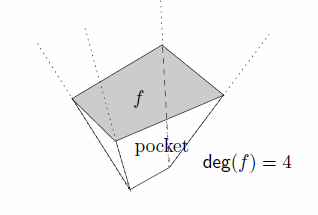
\includegraphics[scale=0.5]{pocket}
\caption{The graph is cited from \cite{har2014epsilon}}
\end{figure}


Now  consider the envelop  as a planar map, which has $|\F|$ faces. 
Define the degree $deg(f)$ as the number of edges of a face $f$. 
Note that, assuming general position, $deg(f)$ is equal to the number of hyperplanes that can be seen from face $f$ (Like Fig. \ref{g1}).
In general, each such plane $g$ seen from $f$ either meets the boundary of $f$ or
	contributes a face to the fully below $f$.
However the latter case is impossible, otherwise, 
	$g$ would not appear on the upper envelope.
 
Let $E$ be the number of edges in the envelop. 
Then by Eular's formula and the fact that $3|\F|\leq 2E$  we have $\sum_{f\in\F} deg(f)\leq 3|\F|-6$. 
Hence, there exist at least $\frac{|\F|}{2}$ faces that have at most $11$ edges, and denote $S^{\leq 11}$ 
	as the set containing such faces. 

For a face in the envelop, define the pocket of $f$ as the set of all halfspaces which contribute to the degree of $f$, i.e. Fig. \ref{g1}. 
Then we have 
\begin{align*}
n&\geq \sum_{f\in \F} (\text{$\sharp$ points contained in the pocket ($f$)})\\
&\geq \sum_{f\in S^{\leq 11}}(\text{$\sharp$ points contained in the pocket ($f$)})\\
&\geq \sum_{f\in S^{\leq 11}}(\epsilon n- 11\beta \epsilon n)\\
&\geq \big|S^{\leq 11}\big|\frac{1}{2}\epsilon n\\
&\geq \frac{1}{4}|\F|\epsilon n
\end{align*}
Thus we have $|\F|\leq \frac{4}{\epsilon}$, which concludes the proof. 



\section{Solve Geometric Set Cover Problem with $\epsilon$-net based methods  }

\begin{problem}
Given a rage space $(X,R)$ with bounded VC dimension, find the minimal subset 
	of $R$ that cover all elements in $X$.
\end{problem}	

First of all, the general version of this problem is NP-Hard (by Meggido in \cite{megiddo1984complexity}.)
Moreover, greedy algorithm can approximately solve the problem within a $O(\log |X|)$ factor,
	 while it has been shown that the problem is NP-Hard to approximate to within a factor of $\Omega(\log |X|)$. 
Then, it raises a natural question whether we can do better on some specific but still useful cases?  

In the following, we can take a subset of the problem where S has a bounded \textit{dual shattering dimension} $\delta^*$,
	and show we can reach a ratio $O(\log \opt)$ on such version, where $\opt$ is the optimal solution to the problem 
	(i.e. the size of the range subset). 

More precisely, given a range space $(X,R)$, we define its dual shattering dimension in the following procedure. 
First of all, for a range space $(X,R)$, we define its dual space as $(R,X^*)$,
	where $\R_p=\{r\in R| p\in r\}$ and $X^*=\{\R_p| p\in X\}$.
Furthermore, the shatter dimension of a space  is the maximum number $\delta$ such that, 
	for any subset $B\subseteq X$,
	$ \big|R_{|B}\big|\leq O(|B|^\delta),$
where $R_{|B}$ is the projection of $R$ on $B$, i.e. $R_{|B}=\{r\cap B| r\in R\}$. 
Then, we conclude that  the dual shattering dimension is the shatter dimension  of dual space 
	of the given $(X,R)$.
 	


\subsection{Unweighted version with $O(\log \opt)$ ratio}
The algorithm \ref{alg-set-cover-unweighted}, designed by Clarkson and Varadarajan \cite{clarkson2007improved}, could
	solve the geometric set cover problem by multiplicative weight methods (MW method, for short). 
The MW method, which has been repeatedly discovered, has been used in many fields 
	including machine learning (Adabost), convex program, online learning and Yao Xor Lemma.
Readers can find a good review of this method in Arora's survey \cite{arora2012multiplicative}.
	
\subsubsection{Algorithm and Intuition}

\begin{algorithm}[h]
	\caption{Hitting set Approx for Unweighted Set Cover}
	\label{alg-set-cover-unweighted}
	Initially, let $w(r) = 1,\forall r\in R$, and let $SOL=\emptyset$\;
	\While{$SOL$ is a set cover}{
		According to the weight, pick a random subset $SOL$ of $R$   of size $O(\frac{\delta^*}{\epsilon} \log \frac{\delta^*}{\epsilon})$\;
		\If{$\exists p\in X$ is uncovered by $SOL$}
		{
			\If{$w(\R_p)\leq \epsilon w(R)$}
				{
					Double the weight for those sets in $R_p$\;
				}
		}
	}%while
	{\bf Return} $SOL$\;
\end{algorithm}

Note that, in each round, by the former discussion, we know the randomly picked set $SOL$ can be a $\epsilon$-net of $(R,X^*)$ with a constant probability. 
If so, then $SOL$ can hit every set $R_p$ with $w(R_p)\geq \epsilon w(R)$ (Here, we actually consider the weighted version of $\epsilon$-net, which
	is easily to be generalized from the original (unweighted) version). 
Thus if $SOL$ is still not a set cover, then the doubling iteration must happen. 
By a well-known argument about MW method, we know the algorithm can perform weight-doubling steps $\opt(\log \opt)$ steps. 
That is, together with the fact that the random sample $SOL$ is an $\epsilon$-net, we bound the number of 
	iterations by $O(\opt\log \opt)$.

Furthermore, instead of constructing $\epsilon$-net by randomly sampling, 
	when we use  $\epsilon$-net with size $O(\frac{1}{\epsilon})$ (e.g. for disks or halfspaces in $\mathbb{R}^3$, shown in Section \ref{first}), 
	we can get a constant-ratio approximation for the problem.
%However, it is not known whether we can beat the above bound for the special case of points and rectangles
%c\cite{har2012weighted}

\subsubsection{Proof}\label{sec:argument}
All that we need to prove is that the algorithm performs at most $\opt(\log \opt)$ weight-doubling steps. 
As we said before, this is a well-known argument, and is also the key to the performance of the algorithm. 

First of all, let $W_0=m$ (total initial weight), where $m$ is the size of $X$.
Then let $W_i$ be the weight at the end of the $i^{th}$ doubling iteration. Note that $W_i$ is called potential function. 

Then we have, 
\begin{equation}\label{eq:bound}
W_i\leq (1+\epsilon)W_{i-1}\leq (1+\epsilon)^im\leq m e^{\epsilon i}.
\end{equation}

Let $t_i(r)$ be the number of times the weight of the  range $r\in R$ was doubled after $i$ doubling iterations.
Then $W_i=\sum_{r\in R} 2^{t_i(r)}$, and \begin{equation}\label{eq:main}
\sum_{r\in \opt} t_i(R)\geq i,
\end{equation} since $\opt$ is the subset intersecting all those sets $R_p$
	which can be doubled. 

By the inequality \eqref{eq:main}, we know $W_i\geq \sum_{r\in \opt} 2^{t_i(r)}\geq \opt \cdot 2^{\frac{i}{\opt}}$ (with a little abuse
	of notations, we use the notation $\opt$ denote both the optimal solution set and its size).
With Eq. \eqref{eq:bound}, we have $m e^{\epsilon i}\geq \opt \cdot 2^{\frac{i}{\opt}}$ and hence $i=O(\opt\log \opt)$.


\renewcommand{\.}{,\ldots,}
%\newcommand{\R}{def
BTW, there is a related note \cite{GeometricSetCover} which writes the same proof in a different way form this note. 
Readers may find more inspiring things from it.  

\subsection{Same $O(\log \opt)$ ratio for weighted version }
First of all, recall that we use reweighting technique and $\epsilon$-net to solve the unweighted version in the above subsection.
Actually, it can be reinterpreted as rounding the LP relaxation. Here we discuss this interpretation. 

Given a range space $(P,R)$ with $P=\{p_1\.p_m\}$ and $R=\{r_1\.r_n\}$,
	 we write its LP relaxation  as follows: \\
	 $\min \sum_{i=1}^{m} y_i~$ $s.t. \sum_{p_j\in r_i} y_i\geq 1, \forall p_j\in P;$
$y_i\geq 0,\forall i\in [m].$

Let $f=\sum_{i=1}^{m} y_i$. Then the LP becomes\\
$\min f~$ $s.t. \sum_{i=1}^{m} \frac{x_i}{f}= 1, \sum_{p_j\in r_i} \frac{x_i}{f}\geq \frac{1}{f}, \forall p_j\in P;$
$x_i\geq 0,\forall i\in [m].$

That is,\\ $\max \epsilon~$ $s.t. \sum_{i=1}^{m} z_i= 1, \sum_{p_j\in r_i} z_i\geq \epsilon, \forall p_j\in P;$
$z_i\geq 0,\forall i\in [m].$

Solve the above LP, we can get a optimal fractional solution $z_1^*\. z_m^*$ and we consider $z_i^*$ as the weight of range $r_i.$
Therefore, consider the dual space $(R,P^*)$ where each range $r_i$ is assigned with a weight $z_i$. 
The $\epsilon$-net of the weighted dual space is a set cover for the original instance. 
In other words, we round the fractional solution $z_1^*\. z_m^*$ by finding an $\epsilon$-net on its weighted dual space. 
Thus we can use known results on the size of $\epsilon$-nets for set systems to immediately derive an approximation.
Armed with this perspective, we can easily extend our $\epsilon$-net based method to weighed version and it 
	can solve the weighed version with same approximation ratio $O(\log \opt)$.

\section{Solve LP with fixed number of variables}

Given a LP with $d$ variables and $n$ constraints, where $d$ is a constant, we want to find its optimal solution as soon as possible. 
There are a lot related  research work on solving the fixed dimension LP. 

In 1991, Seidel proposed an algorithm solving the LP within time $O(d^d n)$ in  \cite{seidel1991small}.
Before Seidel work, Clarkson had proposed an algorithm with running time $O(d^2n+d^d\log n)$. 
Then, Matous$\breve{e}$k, Sharir, and Welzl proposed an algorithm within best time bound $O(d^2n+d^{\sqrt{d\log d}})$ to date,
	which is the same bound as for Kalai's algorithm  by picking random facet. 


In the following, we first give the algorithm \ref{alg:iter}. Then, based on the algorithm \ref{alg:iter}, we give the algorithm \ref{alg:mix} for solving the LP 
	within $O(d^d n)$.

Note that, we still use MW method for solving LP with similar arguments like what we do in the former sections.
Formally,  
let $X$ be the set of variables and  $H$ be the set of constraints and let $\mu():H\rightarrow \mathbb{Z}$ be the weighted function. 
Initially, for each $h\in H$, let $\mu(h)=1$.
Furthermore, for each subset $A\subseteq  H$, denote $\mu(A)$ as  $\sum_{h\in A}\mu(A)$.

\begin{algorithm}[h]
\caption{LP-Iterative}
\label{alg:iter}
Let $V=H$\;
\While{$V\neq \emptyset$}{
\If{$|H|> 6d^2$}{
Choose a random subset $R\subseteq H$ with size $6d^2$\;}
$X_R\leftarrow simplex(R)$\;
$V= \{h\in H|\text{$X_r$ violates $h$ } \}  $\;
\If{$\mu(V)\leq \frac{\mu(H)}{3}d$}{$\forall h\in V, \mu(h)=2\cdot \mu(h)$\;}
}
	{\bf Return} $X_R$\;
\end{algorithm}

With 
a similar argument in the Section \ref{sec:argument}, we can bound the expected number of iterations by $3d\ln n$. 

Formally, let $B$ be the optimal basis and $|B|\leq d$. Then, we still consider the number of doubling iteration happens. 
Note that if $R$ is a $\frac{3}{d}$-net of $(H,X^*)$ and its induced solution $X_R$ is not legal for $H$, then doubling must happen. 
In other words, $  Pr[\text{doulbing interation happens}]\geq Pr[\text{R is an $\epsilon$-net}] \geq 1/2$. 
And after $kd$ rounds, we know the potential function has the bounds:
$$\mu(H)\leq n(1+\frac{1}{3d})^{kd}\leq ne^{\frac{k}{\epsilon}},$$
$$\mu(H)\geq \mu(B)\geq 2k,$$
where we let $\epsilon=\frac{3}{d}$. 
That is the number of doubling iteration is $\leq 3d\ln n$ and hence the running time is $O(d^2n+d^{\sqrt d})$, where 
	the first term of the running time is to compute $d$ and the second term is for running simplex algorithm. 

\begin{algorithm}[h]
	\caption{LP-MIXED}
	\label{alg:mix}
	Let $V^*=\emptyset, V=H, C_d=9d^2$\;
	\While{$V\neq \emptyset$}{
	\If{$|H|\leq C_d$}
	{
		Choose a random subset $R\subseteq H\setminus V^*$ with size $d\sqrt n$\;
		$X^*\leftarrow$ LP-Iterative($R\cup V^*$ )\;
	    $V= \{h\in H|\text{$X^*$ violates $h$} \} $\;
	    \If{$|V|\leq 2\sqrt{n}$}
	    {$V^*=V^*\cup V$\;}
	   }
	  }
	{\bf Return} $X^*$\;
\end{algorithm}

Similarly, for algorithm \ref{alg:mix}, it can be concluded that the expected number of successful iteration  is bounded by $d$. 
Let $B^*$ be the optimal basis and in each iteration, some $h\in B^*$ should be added to $V$ (thus to $V^*$). 
Thus $Pr[\text{The current iteration is successful}]\geq 1/2$ and hence the running time is 
	bounded by $2(d+1)T_{iterative}(\sqrt{C_dn})+O(d^2 n)$, where the latter term in running time
	is for testing violation.
\cite{Seidel}
\bibliographystyle{plain}
\bibliography{a}
%% To add references, uncomment the following two lines and
%% add the relevant bibitems.

\end{document} 